\documentclass[a0,landscape]{a0poster}

%%%%%%%%%%%%%%%%%%%%%%%%%%%%%%%%%%%%%%%%%%%%%%%%%%%%%%%%%%%%%%%%%%%%%%%
% Paket zum Erzeugen der Spalten
\usepackage{multicol}

%%%%%%%%%%%%%%%%%%%%%%%%%%%%%%%%%%%%%%%%%%%%%%%%%%%%%%%%%%%%%%%%%%%%%%%
% Eingabekodierung
\usepackage[ansinew]{inputenc}
\usepackage[T1]{fontenc}
\usepackage{ae} %wenn Ulaute nicht gehen

%\newcommand{\changefont}[3]{\fontfamily{#1} \fontseries{#2} \fontshape{#3} \selectfont}

\usepackage[ngerman]{babel}
%\begin{�bler Trick um die Orinal�berschrift zu unterdr�cken}
\addto{\captionsngerman}{\renewcommand*{\refname}{}} %Literatur�berschfit unterdr�cken
%\ende{�bler Trick}

%%%%%%%%%%%%%%%%%%%%%%%%%%%%%%%%%%%%%%%%%%%%%%%%%%%%%%%%%%%%%%%%%%%%%%%
% f�r Farbe
\usepackage{color} 
\definecolor{darkgreen}{rgb}{0,0.5,0} 
\definecolor{darkblue}{rgb}{0,0,0.5}

%%%%%%%%%%%%%%%%%%%%%%%%%%%%%%%%%%%%%%%%%%%%%%%%%%%%%%%%%%%%%%%%%%%%%%%
% Mathepaket
\usepackage{amsmath} 

%%%%%%%%%%%%%%%%%%%%%%%%%%%%%%%%%%%%%%%%%%%%%%%%%%%%%%%%%%%%%%%%%%%%%%%
% Ist f�r Boxen (wie das hier benutzte Ovalbox) zust�ndig
\usepackage{fancybox}

%%%%%%%%%%%%%%%%%%%%%%%%%%%%%%%%%%%%%%%%%%%%%%%%%%%%%%%%%%%%%%%%%%%%%%%
% Graphikpaket, erm�glicht png, jpg und pdf bilder
\usepackage{graphicx}

%%%%%%%%%%%%%%%%%%%%%%%%%%%%%%%%%%%%%%%%%%%%%%%%%%%%%%%%%%%%%%%%%%%%%%%
% Seiteneinstellungen
\renewcommand\baselinestretch{1.35}
\parskip=0.5\baselineskip

\parindent0mm %Einr�cktiefe der ersten Zeile eines Absatzes
\topmargin-28pt
\marginparwidth0mm

%R�nder rechts/links
\oddsidemargin-13pt
\evensidemargin-13pt
\textwidth1130mm
\textheight785mm


%%%%%%%%%%%%%%%%%%%%%%%%%%%%%%%%%%%%%%%%%%%%%%%%%%%%%%%%%%%%%%%%%%%%%%%
% Eigene Definitionen zur Erleichterung des Satzes
\newcommand{\spaltenbreite}{15}   % Spaltenbreite f�r Bilder
\newcommand{\bildbreite}{15cm}    % Einheitliche Bildbreite

%%%%%%%%%%%%%%%%%%%%%%%%%%%%%%%%%%%%%%%%%%%%%%%%%%%%%%%%%%%%%%%%%%%%%%%
% Box- und Spalteneinstellungen
\setlength{\fboxrule}{3.25mm} %Definiert die Linienst�rke f�r nachfolgende fbox- und framebox-Befehle
\setlength{\fboxsep}{5mm} %Abstand zwischen Rahmen und Text bei den /fbox und /framebox Befehlen.
\setlength{\columnsep}{15mm}     %Spaltenabstand
\setlength{\columnseprule}{3pt}  %Balken zwischen Spalten {0pt}->keine Balken

%%%%%%%%%%%%%%%%%%%%%%%%%%%%%%%%%%%%%%%%%%%%%%%%%%%%%%%%%%%%%%%%%%%%%%%
% Einheitsl�nge f�r picture-Umgebungen
%\setlength{\unitlength}{1.0cm}
\unitlength1cm

%%%%%%%%%%%%%%%%%%%%%%%%%%%%%%%%%%%%%%%%%%%%%%%%%%%%%%%%%%%%%%%%%%%%%%%
% Grafikpfad, hier liegen alle Bilder
%\graphicspath{{images/}}

%%%%%%%%%%%%%%%%%%%%%%%%%%%%%%%%%%%%%%%%%%%%%%%%%%%%%%%%%%%%%%%%%%%%%%%
% Zaehler fuer lineale. Sie werden gebraucht, wenn das Linealmacro
% included wird
\newcounter{skalax}
\newcounter{skalay}


\begin{document}

\pagecolor[rgb]{1.0,1.0,0.82}
%\changefont{cmr}{bx}{n}
%\changefont{cmtt}{m}{n}

%%%%%%%%%%%%%%%%%%%%%%%%%%%%%%%%%%%%%%%%%%%%%%%%%%%%%%%%%%%%%%%%%%%%%%%
% Kopf, hier funktioniert alles mit 'put'
%%%%%%%%%%%%%%%%%%%%%%%%%%%%%%%%%%%%%%%%%%%%%%%%%%%%%%%%%%%%%%%%%%%%%%%

\framebox[1145mm]
{
  \begin{Bcenter} % centering for boxes

  % Logos einbinden (per Hand plazieren)
  \begin{picture}(0,0)
    \put(44.8 , -8.0){
\includegraphics[height=80mm]{tu.jpg}}
    \put(46.9 ,-9.2){\LARGE \textsf{\textbf{TU Berlin}}}
    \put(-50.0, -8.0){
\includegraphics[height=80mm]{bccn.pdf}}
    \put(-56.0,-9.2){\large \textsf{\textbf{Bernstein Center for Computational Neuroscience}}}
  \end{picture}

  \\[0.02\textheight]
  \textbf{{\huge Implementation and Evaluation of the}}\\[0.006\textheight]
  {\huge \textrm{\textbf{Unified Visual Attention Model (UVAM)}}}\\[0.004\textheight]
  \\[0.004\textheight]
  {\LARGE \textbf{Alexander Schlegel, Rafael Schultze-Kraft}}\\[0.004\textheight]
  {\today}

\end{Bcenter}
}
%%%%%%%%%%%%%%%%%%%%%%%%%%%%%%%%%%%%%%%%%%%%%%%%%%%%%%%%%%%%%%%%%%%%%%%
% Einstellung des Eckenradius' der ovalen Boxen (\Ovalbox)
\cornersize*{80mm}


\linethickness{0.1mm}
\setlength{\fboxrule}{2.25mm}

    \vspace*{0.018\textheight}

%%%%%%%%%%%%%%%%%%%%%%%%%%%%%%%%%%%%%%%%%%%%%%%%%%%%%%%%%%%%%%%%%%%%%%% 
% neuer Kasten
%\Ovalbox
%{
  \parbox{\textwidth}{
    \begin{multicols}{4}
      
      \begin{center} \textbf{\Large Introduction} \end{center}
\doublespacing
Object recognition in machines faces the problem that it requires complex calculations and therefore real-time performances are difficult to achieve. Visual attention has shown to be a good mechanism to improve the runtime of object recognition by rapidly filtering interesting image regions likely to contain significant information for a detailed analysis. Thereby the need for computational resources are reduced and the object recognition procedure is speeded up.\par
In the present work we implemented and evaluated the Unified Visual Attention Model (UVAM), first introduced by \cite{lee2010}. The UVAM is based on the Shift Invariant Feature Transform (SIFT) \cite{lowe2004}, a popular approach in objected recognition based on local features. In addition the UVAM makes use of bottom-up and top-down computational models of attention to speed up the object recognition procedure. For bottom-up attention we used the saliency based computational model by Itti et al. \cite{itti1998}, where regions of an image are marked as salient with respect to their corresponding low-level features. As a metric for top-down attention Lee et. al \cite{lee2010} introduced the concept of 'familiarity': Familiarity is a measure of the resemblance of local features extracted from the input image to features of trained object models stored in a database. Features of high familiarity are seen as evidence of object existence, and are used to guide attention to locations likely to contain the corresponding object. Both saliency and familiarity map are combined to the unified attention map, that is used to guide attention for detailed analysis of the input image. The outline of the proposed UVAM is shown in Fig. 1. The top-down and bottom-up components of the UVAM can be divided into two stages: the feed-forward attention stage of the left hand side, and the attention feedback loop of the right hand side. The feed-forward
attention stage provides a preliminary estimation of the location of trained objects before starting the detailed object recognition. The attention feedback loop updates this estimation later based on the results of detailed object recognition on each selected ROI. The bottom-up saliency map (S-map) is calculated once during the feed-forward attention stage. In contrast, top-down familiarity is calculated once during the feed-forward attention stage to obtain the feed-forward familiarity map (FF F-map), and then repeatedly during the attention–recognition feedback loop to obtain the feedback familiarity map (FB F-map). The S-map and the two F-maps are combined into the unified attention map (UA-map), which is used to select the ROI for detailed object recognition.\\
\begin{center}
	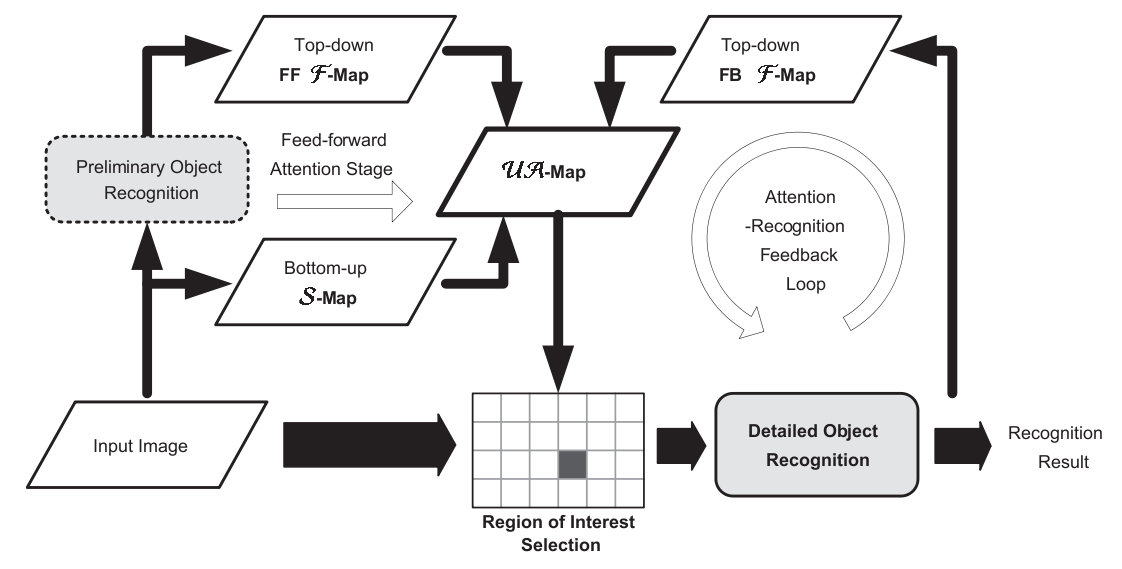
\includegraphics[scale=0.65]{alg.png}
	\caption{Fig.1: Outline of the UVAM algorithm.}
	\label{fig:1}
\end{center}



      \begin{center} \textbf{\Large Experiments} \end{center}
To evaluate the UVAM algorithm we used the Columbia Object Image Library (COIL-100, http://www1.cs.columbia.edu/CAVE/software/softlib/coil-100.php). Therefor we extracted the 75 first objects containing the largest amount of keypoints and neglected all others. In addition, we only used objects without rotation. These objects were embedded into backgrounds taken from the McGill Calibrated Colour Image Database (http://tabby.vision.mcgill.ca/). An example test image is illustrated in Fig. 2.\\
\begin{center}
	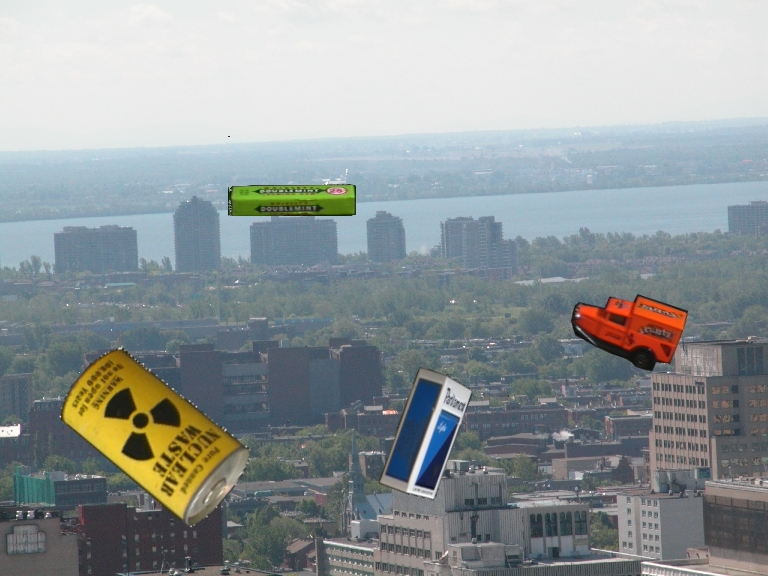
\includegraphics[scale=1.00]{img01.jpg}
	\caption{Fig. 2: An example of a test image using COIL-100 objects embedded into a background.}
	\label{fig:2}
\end{center}
To assess the performance of the UVAM algorithm and compare it, our testing procedure contained four different steps: First, we tested speed performance without the use of neither bottom-up saliency nor familiarity maps. Second, we incorporated only saliency maps into the algortihm. Third, we used only familiarity maps to test the performance. And finally, we used the actual UVAM algorithm (including both saliency and familiarity maps) to assess the speed performance of the object recognition process. 


      \begin{center} \textbf{\Large Results} \end{center}

      \begin{center} \textbf{\Large Conclusion} \end{center}

      %%%%%%%%%%%%%%%%%%%%%%%%%%%%%%%%%%%%%%%%%%%%%%%%%%%%%%%%%%%%%%%%%%%%%%%
% Literaturverzeichnis

%\begin{�bler Trick um die Orinal�berschrift zu unterdr�cken}
\vspace*{1cm}
      \begin{center} \textbf{\Large References} \end{center}
\vspace*{-4.5cm}
%\end{�bler Trick}

\renewcommand{\baselinestretch}{1.05}\small\normalsize
\begin{thebibliography}{9}
\bibitem{lee2010} \textsc{S. Lee, K. Kim, J.-Y. Kim, M. Kim, H.-J. Yoo,} ``Familiarity based unified visual attention model for fast and robust object recognition'', \textsl{Pattern Recognition} 43, 2010.

\bibitem{lowe2004} \textsc{D. G. Lowe,} ``Distinctive Image Features from Scale-Invariant Keypoints'', \textsl{nternational Journal of Computer Vision} 60, 2004.

\bibitem{itti1998} \textsc{L. Itti, C. Koch \& E. Niebur,}  ``A Model of Saliency-Based Visual Attention for Rapid Scene Analysis'',  \textsl{IEEE Transactions on Pattern Aanalysis and Machine Intelligence} 20, 1998.

\end{thebibliography}

     
    \end{multicols}
  }
%}



\end{document}
